\chapter{Introdução}
\label{cap:introducao}

Um dos principais elementos em um sistema de automação, geralmente associado a um \acrlong{CLP}(\acrshort{CLP}), é uma \acrlong{IHM} (\acrshort{IHM}) e tem a função de transformar ou traduzir dados complexos em uma interface acessivel à operação do sistema. 

A \acrshort{IHM} é um equipamento composto por uma tela, alfanumérica ou gráfica, para exibição de status de processo, gráficos e indicadores de desempenho, alertas, diagnóstico de problemas entre outras informações e também um conjunto de teclas para acionamentos, ajuste de parâmetros e navegação. Em alguns casos a tela gráfica possui uma camada sensível ao toque (\textit{touchscreen}).

O uso de \acrshort{IHM} traz diversas vantagens ao processo, planta ou sistema, pois permite um alto grau de personalização, uma fácil configuração, a implementação de controle de acesso, diversas possibilidades de conexão, o monitoramento eficiente dos processos, o diagnóstico de problemas, a exibição de indicadores de desempenho bem como armazenamento de receitas de operação e alteração de parâmetros mediante a tomada de decisão dos operadores. 

Praticamente todos os distribuidores ou desenvolvedores de equipamentos para automação industrial possuem suas próprias \acrshort{IHM}s e \acrshort{CLP}s, podemos destacar na Figura \ref{fig-altus_duo} um equipamento da linha DUO, que integra os dois equipamentos em um só, desenvolvido pela empresa nacional Altus Sistemas de Automação S.A.

\begin{figure}[h!]
	\centering
	\Caption{\label{fig-altus_duo} CLP com IHM integrada - Altus Série DUO}		
	\IBGEtab{}{
		\fbox{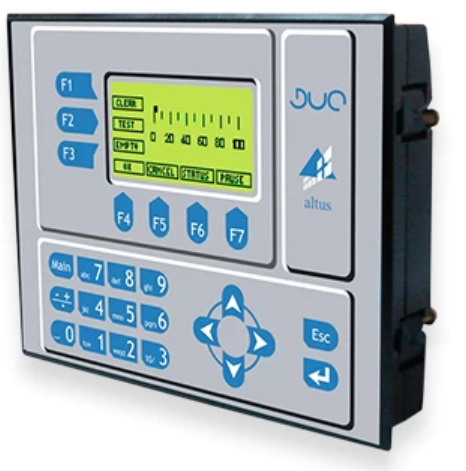
\includegraphics[scale=0.7]{figuras/altus_duo}}
	}{
		\Fonte{Altus}
	}
\end{figure}


A \textbf{série iX} é outra linha de produtos da Altus que é composta por um conjunto de \acrshort{IHM}s utilizadas como terminais de operação e visualização para aplicações industriais. É uma plataforma aberta, podendo interagir com ferramentas .NET, além da versatilidade das suas aplicações, desenvolvidas através da interface iX Developer, que podem ser executados em vários modelos de IHM dentro da mesma série.

\begin{figure}[h!]
	\centering
	\Caption{\label{fig-altus_ix_series}\acrlong{IHM} (\acrshort{IHM}) - Altus Série iX}		
	\UECEtab{}{
		\fbox{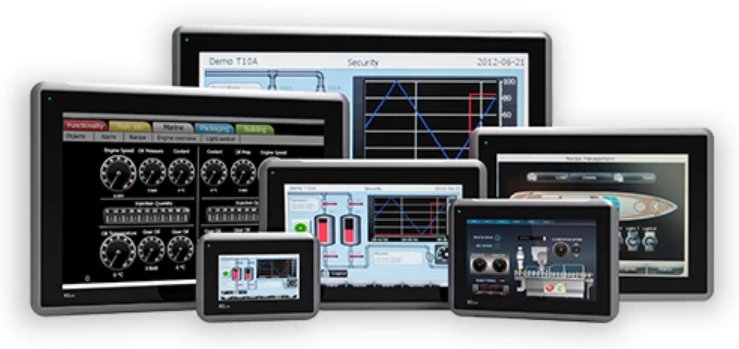
\includegraphics[scale=0.8]{figuras/altus_ix_series}}
	}{
		\Fonte{Altus}
	}
\end{figure}

A série iX bem como outras linhas de IHM, são denominadas pelo fabricante/fornecedor como Terminais Gráficos, funcionalmente menos abrangente, mas para nosso uso, equivalente. 


Os terminais que compõem a série são: iX-T4A, iX-T7A, iX-T10A, iX-T5F-2, iX-T7F-2 e iX-T10F-2, sendo eles terminais gráficos, coloridos, \textit{touchscreen} e display com tecnologia TFT \footnote{Transistor de Película Fina \cite{tecnoblog_tft}. }
De acordo com o fornecedor, este série foi descontinuada, assim, não são mais fabricados ou disponibilizados para venda ou mesmo suporte técnico. A sugestão para reposição são os teminais da linha X2-BASE, que são integralmente compatíveis com a série iX \cite{ix_t7f_2-x2_base_7}.


\section{Motivação}
\label{sec:motivacao}

A disponibilidade de equipamentos no laboratório de controle de processos, especificamente o terminal gráfico iX-T7F-2 e o CLP da Série DUO, montado em um kit didático (\acrlong{TB} - TB131), e a ausência de um procedimento de trabalho, contendo o passo-a-passo para conexão com outros equipamentos como \acrshort{CLP}s, juntamente com a necessidade da produção de um projeto de férias, motivaram a produção deste trabalho, facilitando a consolidação das competências adquiridas quanto ao uso do referido equipamento e suas utilizações nos cursos de Engenharia de Controle e Automaçãoe e Técnico em Automação Industrial.  




\section{Objetivos}
\label{sec:objetivos}


\subsection{Objetivo Geral}
\label{sec:objetivo-geral}

Proporcionar suporte básico à comunicação entre \acrshort{IHM} e \acrshort{CLP} alocados no laboratório de Controle de Processos, bem como uma atividade guiada simples para introdução à sua utilização.




\subsection{Objetivos Específicos}
\label{sec:objetivos-especificos}


	\begin{alineas}
		\item Especificar a forma de conexão entre equipamentos:
			\begin{alineas}
			\item terminal gráfico (iX-T7F-2) e \acrshort{CLP} (\acrshort{TB}131);
			\item para a transferência da aplicação(projeto) entre o computador e o terminal gráfico.
			\end{alineas}
		\item Introdução à utilização do terminal gráfico iX-T7F-2;
		\item Aplicação de comunicação entre \acrshort{CLP} (\acrshort{TB}131) e \acrshort{IHM} (ix-T7F-2).
	\end{alineas}
